% This work is licensed under the Creative Commons
% Attribution-NonCommercial-ShareAlike 4.0 International License. To view a copy
% of this license, visit http://creativecommons.org/licenses/by-nc-sa/4.0/ or
% send a letter to Creative Commons, PO Box 1866, Mountain View, CA 94042, USA.

\subsection{Triangulation}

\Large{ $B_h$ oder $B_b$ ???}

\begin{definition_}
	Let $\Omega \subset \R^d$ ($d \geq 1$) bounded domain. A partition $T_h$ of $\Omega$ with $\tau \in T_h$ is a \textit{triangulation} if
	\begin{enumerate}[label=\alph*)]
		\item $\forall \tau \in T_h$, $\tau$ is closed, $\tau^0 \neq \emptyset$, $\tau$ is connected and $\partial \tau \in C^{0,1}$
		\begin{figure}[h!]
	\center

	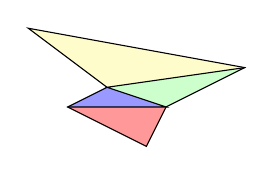
\begin{tikzpicture}[scale=1]
	
	
	% fill triangles
	\fill[red!40!white]   (0,0) -- ++(1,-0.5) -- ++(0.25,0.5) --cycle;
	\fill[blue!40!white]  (0,0) -- ++(1.25,0) --++(-0.75,0.25) --cycle;
	\fill[green!20!white]   (1.25,0) --++(-0.75,0.25) --++(1.75,0.25) --cycle;
	\fill[yellow!20!white]   (0.5,0.25) --++(1.75,0.25) --  ++(-2.75,0.5) --cycle;
	
	% outline
	\draw (0,0) -- ++(1,-0.5) -- ++(0.25,0.5)-- ++(1,0.5) -- ++(-2.75,0.5)-- ++(1,-0.75)--cycle;
	
	% this is unrobust
	\draw (0,0) -- ++(1.25,0) --++(-0.75,0.25) --++(1.75,0.25);
	
 	%\node at (1,-1) {example triangulation,};
	%\node at (1,-1.4) {$\tau$ disjunct};
	\end{tikzpicture}
		
\caption{example triangulation, $\tau$ disjunct}
\label{ch2_example_triang}

\end{figure}		
		\item $\bigcup \limits_{\tau \in T_h} = \overline{\Omega}$
		
		\item $\forall \tau_1,\tau_2 \in T_h:$ $\tau^0_1\cap \tau^0_2 = \emptyset$
	\end{enumerate}

	\begin{align*}
		h_{\tau} &= \diam (\tau)\\
		h &= \underset{\tau \in T_h}{\max} h_{\tau}\\
		\rho_{\tau} &= \underset{\tau \in T_h}{\sup} \{2r: B_r \subset \tau, d\text{-ball of radius  }r \} \\
		\rho &= \underset{\tau \in T_h}{\max} \rho_{\tau}
	\end{align*}
\end{definition_}
%TODO add picture

We further require that all faces of $\tau_i \in T_h$ are faces of $\tau_i \in T_h$ or part of $\partial \Omega$.
\begin{figure}[h!]
	\center


	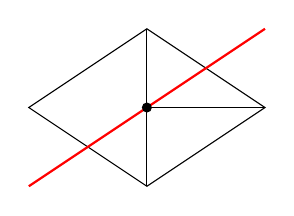
\begin{tikzpicture}[scale=1]

	% outline
	\draw (0,0) -- ++(1.5,-1) -- ++(1.5,1)-- ++(-1.5,1) -- cycle;
	\draw (1.5,-1) -- ++(0,2);
	\draw (1.5,0) -- ++(1.5,0);
	
	% red cross
	\draw[thick,red] (0,-1) --++ (3,2);

	% dot middle
	\filldraw (1.5,0) circle (1.6pt);

	\end{tikzpicture}

	\caption{not allowed}
	\label{ch1_triang_not_allowed}

\end{figure}
Hanging nodes cannot guarantee continuity of functions.

$T_h$ triangulation of $\Omega$ with Lagrange elements $(\tau,P_\tau,\Sigma_\tau)$ with $\tau \in T_h$\\
$ N_h$ is set of all vertices of $T_h$. For $b\in N_0 $ $T_h(b) $ is the set of all finite elements, for which $b$ is a vertex.

\begin{definition_}
	(Finite elements space)
	\begin{equation*}
		X_h = \left \{ v = (v_\tau)_{\tau \in T_h} \in \prod \limits_{\tau \in T_h} P_\tau \left|
\begin{array}{c}
\forall b  \in\N_h : \forall \tau_1,\tau_2 \in T_h(b):\\
B_{b,\tau_1}(v_{\tau_1}) = B_{b,\tau_2}(v_{\tau_2}) 
\end{array}		
 \right.\right \}
	\end{equation*}
\end{definition_}
For Lagrange elements:
\begin{equation*}
	v_{\tau_1}(b) = B_{b,\tau_1}(v_{\tau_1}) = B_{b,\tau_2}(v_{\tau_2}) = v_{\tau_2}(b)
\end{equation*}

Functions on $X_h$ are uniquely determined by $\{v(b): b \in N_h \}$ we thus also have 
\begin{align*}
	X_h = \Big \{& v: \overline{\Omega} \to \R,\ \forall \tau \in T_h, v|_\tau \in P_\tau \text{ and }\\ &{} \quad \forall b \in N_h: \forall \tau_1,\tau_2 \in T_h(b) ,\ B_{b,\tau_1}(v|_{\tau_1}) = B_{b,\tau_2}(v|_{\tau_2})  \Big\}.
\end{align*}

\begin{example}
	linear lagrange elements $a_i$ vertex of $\tau \in T_h$,
	\begin{align*}
		B_{i,\tau}(p)  &= p(a_i) \quad \forall p \in P_\tau \\
		X_h &= \{ v:\overline{\Omega} \to \R : \forall \tau \in T_h, v|_{\tau} \in P_1(\tau) ,\ v \text{ continuous in } \overline{\Omega} \}
	\end{align*}
\end{example}

$X_h$ is a finite dimensional space, has a basis
\begin{equation*}
	\Sigma_h = \{ B_{h,j} : j= 1,\dots,N  \} \quad \text{ set of DoFs} 
\end{equation*}

$\varphi_i \in X_h\ i=1,\dots,N$ with $B_{h,j}(\varphi_i) = \delta_{ij} \quad i,j=1,\dots,N$ (global basis funktions),$\varphi_i \in C^0(\overline{\Omega})$, $\forall \tau \in T_h: \varphi_i|_\tau \in P_i(\tau)$. $\varphi_i(b_j) = \delta_{ij}$ for $i,j = 1,\dots,N$ with $b_j \in N_h$ vertices of all $\tau \in T_h$.\nl
\centering
\begin{tabular}{c|c}
	global  & local \\ \hline 
	&\\
	$\overline{\Omega} $&  ($\tau , P_\tau, \Sigma_\tau$) \\
	$X_h$ & $P_\tau = \{ v|_\tau :v \in X_h  \}$ \\
	global basis $\varphi_1,\dots,\varphi_N$ & local basis $p_1,\dots,p_N$ on $\tau$\\
	$\Sigma_h$ Dofs on $X$ & $\Sigma_\tau$ DoFs on $\tau$\\
	$b_1,\dots,b_N$ vertices of $\overline{\Omega}$ & $a_1,\dots,a_N$ vertices on $\tau$		
\end{tabular}
%%%TODO fix distances 

\begin{example}
	\begin{align*}
		- \laplace u &=1 \quad \tin \overline{\Omega} \subset \R\\
		u &=0 \quad \ton \partial \Omega
	\end{align*}
	\begin{equation*}
		a(u,v) = \int \limits_\Omega  \nabla u \cdot \nabla v \diff c = \int \limits_\Omega v\diff x = F(v) \quad \forall v \in H^1_0(\Omega)
	\end{equation*}
	\begin{align*}
		V_h &= \{ u \in X_h, u=0 \ton \partial \Omega  \}\\
			&= \{ u: \overline{\Omega} \to \R , \ u \text{ piecewise linear }, u=0 \ton \partial \Omega   \}
	\end{align*}
	$\varphi_1,\dots,\varphi_N$ global basis functions of $V_h$.
	\begin{equation*}
		a(\varphi_i,\varphi_j) = \int \limits_\Omega \nabla \varphi_i \cdot \nabla \varphi_j = 
		\begin{cases}
		\text{const} & \text{ if } a_i,a_j \text{ in some triangle}\\
		0 & \text{otherwise}
		\end{cases}
	\end{equation*}
	$\Omega = (-1,1)^2$, $h = \frac{1}{2}$.
	\begin{figure}[h!]
	\center
	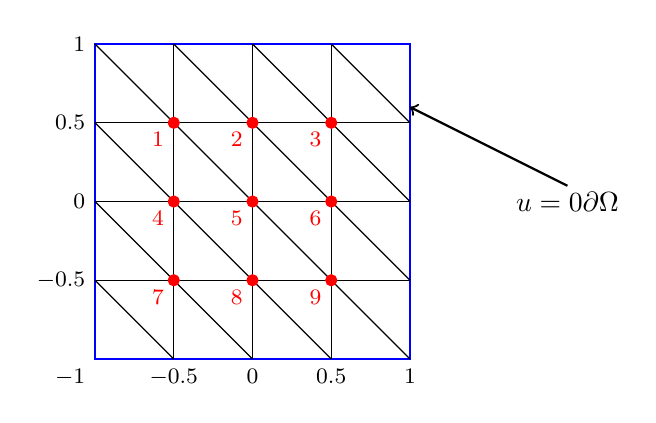
\begin{tikzpicture}[scale=2]
	
	\pgfmathsetmacro{\zerox}{-1}
	\pgfmathsetmacro{\zeroy}{-1}
	
	\draw[blue] (\zerox,\zeroy) -- ++(2,0)-- ++(0,2) --++(-2,0) --cycle;
	
	%vertical lines
	\draw (\zerox,\zeroy) ++(0.5,0)-- ++(0,2);
	\draw (\zerox,\zeroy) ++(1,0)-- ++(0,2);
	\draw (\zerox,\zeroy) ++(1.5,0)-- ++(0,2);
	
	% horizontal lines
	\draw (\zerox,\zeroy) ++(0,0.5)-- ++(2,0);
	\draw (\zerox,\zeroy) ++(0,1)-- ++(2,0);
	\draw (\zerox,\zeroy) ++(0,1.5)-- ++(2,0);
	
	% diagonal lines
	\draw (\zerox,\zeroy) ++(0,0.5)-- ++(0.5,-0.5);
	\draw (\zerox,\zeroy) ++(0,1)-- ++(1,-1);
	\draw (\zerox,\zeroy) ++(0,1.5)-- ++(1.5,-1.5);
	\draw (\zerox,\zeroy) ++(0,2)-- ++(2,-2);
	\draw (\zerox,\zeroy) ++(0.5,2)-- ++(1.5,-1.5);
	\draw (\zerox,\zeroy) ++(1,2)-- ++(1,-1);
	\draw (\zerox,\zeroy) ++(1.5,2)-- ++(0.5,-0.5);
	
	
	% inner points
	\filldraw[red]  (\zerox,\zeroy) ++ (0.5,0.5) circle (1pt)
					(\zerox,\zeroy) ++ (0.5,1) circle (1pt)
					(\zerox,\zeroy) ++ (0.5,1.5) circle (1pt)
					(\zerox,\zeroy) ++ (1,0.5) circle (1pt)
					(\zerox,\zeroy) ++ (1,1) circle (1pt)
					(\zerox,\zeroy) ++ (1,1.5) circle (1pt)
					(\zerox,\zeroy) ++ (1.5,0.5) circle (1pt)
					(\zerox,\zeroy) ++ (1.5,1) circle (1pt)
					(\zerox,\zeroy) ++ (1.5,1.5) circle (1pt);
	
	
	
	\fill[red,font=\footnotesize] (\zerox,\zeroy) ++ (0.5,1.5)  node[below left] {$1$}
								  (\zerox,\zeroy) ++ (1,1.5)  node[below left] {$2$}
								  (\zerox,\zeroy) ++ (1.5,1.5)  node[below left] {$3$}
								  (\zerox,\zeroy) ++ (0.5,1)  node[below left] {$4$}
								  (\zerox,\zeroy) ++ (1,1)  node[below left] {$5$}
								  (\zerox,\zeroy) ++ (1.5,1)  node[below left] {$6$}
								  (\zerox,\zeroy) ++ (0.5,0.5)  node[below left] {$7$}
								  (\zerox,\zeroy) ++ (1,0.5)  node[below left] {$8$}
								  (\zerox,\zeroy) ++ (1.5,0.5)  node[below left] {$9$};
	
	
	% axis numbering
	\fill[black,font=\footnotesize] (\zerox,\zeroy)  node[below left] {$-1$}
									(\zerox,\zeroy) ++(0.5,0) node[below] {$-0.5$}
									(\zerox,\zeroy) ++(1,0) node[below] {$0$}
									(\zerox,\zeroy) ++(1.5,0) node[below] {$0.5$}
									(\zerox,\zeroy) ++(2,0) node[below] {$1$}
									
									(\zerox,\zeroy) ++(0,0.5) node[left] {$-0.5$}
									(\zerox,\zeroy) ++(0,1) node[left] {$0$}
									(\zerox,\zeroy) ++(0,1.5) node[left] {$0.5$}
									(\zerox,\zeroy) ++(0,2) node[left] {$1$};
									
   	\node at (\zerox + 3,\zeroy + 1) {$u=0 \ton \partial \Omega$};
   	\draw[thick,-to] (\zerox + 3 ,\zeroy + 1.1) -- ++(-1,0.5);							    
	
	\end{tikzpicture}
		
	\caption{meshed $\Omega $}\label{tikz/chapter2/mesh_omega}
	\label{ch2_mesh_omega}

\end{figure}\\
	Define $F$ as follows
	\begin{align*}
		&{} F\colon \hat{\tau} \to \tau \quad F(x,y) = h \begin{pmatrix} x\\ y \end{pmatrix} + a_1\\
		&{} F^{-1}\colon \tau \to \hat{\tau} \quad F^{-1}(x,y) = h^{-1} \left ( \begin{pmatrix}x \\ y \end{pmatrix} - a_1 \right )
	\end{align*}
	
	
\begin{figure}[H]
	\center
	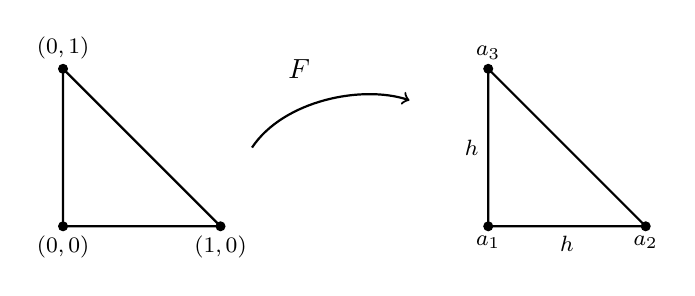
\begin{tikzpicture}[scale=2]
	
	
	% first simplex
	\draw[thick] (0,0) -- ++(0,1) -- ++(1,-1)--cycle;
	\filldraw (0,0)         circle (0.8pt)
			  (0,0) ++(1,0) circle (0.8pt)
			  (0,0) ++(0,1) circle (0.8pt);
	\fill[black,font=\footnotesize] (0,0) node[below] {$(0,0)$}
									(0,0) ++(1,0) node[below] {$(1,0)$}
									(0,0) ++(0,1) node[above] {$(0,1)$};
	
	%arrow
	\draw[thick,-to] (1.2,0.5) .. controls (1.4,0.8) and (1.9,0.9) .. (2.2, 0.8);
	
	%second simplex							
	\draw[thick] (0,0) ++ (2.7,0) -- ++(0,1) -- ++(1,-1)--cycle;
	\filldraw 	(0,0) ++ (2.7,0)         circle (0.8pt)
				(0,0) ++ (2.7,0) ++(1,0) circle (0.8pt)
				(0,0) ++ (2.7,0) ++(0,1) circle (0.8pt);
	%\filldraw (2.2,0)         circle (0.8pt)
	%		  (2.2,0) ++(2,0) circle (0.8pt)
	%		  (2.2,0) ++(1,1) circle (0.8pt);
	\fill[black,font=\footnotesize] (2.7,0) node[below] {$a_1$}
									(2.7,0) ++(1,0) node[below] {$a_2$}
									(2.7,0) ++(0,1) node[above] {$a_3$};								
			
	
	
	%\draw (2.2,0) ++(45:.6) arc (45:0:.6);
	
	
	\node at (1.5,1) {$F$};
	\fill[black,font=\footnotesize] (3.2,0)  node[below] {$h$}
									(2.7,0.5) node[left] {$h$};
	\end{tikzpicture}
	
	\caption{$F:\hat{\tau} \to \tau $}
	\label{ch2_plot_f}
	
\end{figure}
	
	\begin{align*}
		&\text{basis functions on } \hat{\tau} &&  \text{ basis functions on } \tau\\
		&\begin{rcases}
		&\hat{P}_1(x,y)=1-x-y \\
		&\hat{P}_2(x,y)=x \\
		&\hat{P}_3(x,y)=y \\
		\end{rcases}  \text{ for } (\hat{x},\hat{y}) \in \hat{\tau} \implies &&
		\begin{cases}
		P_1(x,y) = 1- \frac{x-x_1}{h} - \frac{y-y_1}{h} \\
		P_2(x,y) = \frac{x-x_1}{h} \\
		P_3(x,y) = \frac{y-y_1}{h} \\
		\end{cases}
	\end{align*}
	implies 
	\begin{equation*}
		A_{ij} =(a(\varphi_i, \varphi_j)) \in \R^{9 \times 9} 
	\end{equation*}
	
	\begin{figure}[h!]
	\center
	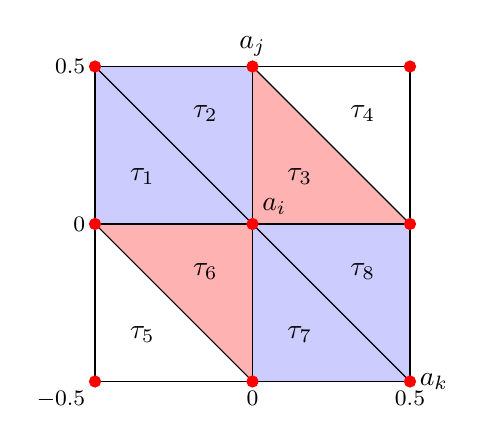
\begin{tikzpicture}[scale=2]
	
	\pgfmathsetmacro{\zerox}{-1}
	\pgfmathsetmacro{\zeroy}{-1}
	
	%color the important triangles
	\fill[red!30!] (\zerox,\zeroy) ++ (1,1) -- ++(0,-1) -- ++(-1,+1) --cycle;
	\fill[red!30!] (\zerox,\zeroy) ++ (1,1) -- ++(0,1) -- ++(1,-1) --cycle;
	
	\fill[blue!20!] (\zerox,\zeroy) ++ (1,1) -- ++(-1,0) -- ++(0,+1) -- ++(1,0) --cycle;
	\fill[blue!20!] (\zerox,\zeroy) ++ (1,1) -- ++(1,0) -- ++(0,-1) -- ++(-1,0) --cycle;
	
	% draw outline
	\draw (\zerox,\zeroy) -- ++(2,0)-- ++(0,2) --++(-2,0) --cycle;
	
	%vertical lines
	\draw (\zerox,\zeroy) ++(1,0)-- ++(0,2);
	
	% horizontal lines
	\draw (\zerox,\zeroy) ++(0,1)-- ++(2,0);

	
	% diagonal lines
	\draw (\zerox,\zeroy) ++(0,1)-- ++(1,-1);
	\draw (\zerox,\zeroy) ++(0,2)-- ++(2,-2);
	\draw (\zerox,\zeroy) ++(1,2)-- ++(1,-1);
	
	
	% inner points
	\filldraw[red]  (\zerox,\zeroy) circle (1pt)
					(\zerox,\zeroy) ++ (0,1) circle (1pt)
					(\zerox,\zeroy) ++ (0,2) circle (1pt)
					(\zerox,\zeroy) ++ (1,0) circle (1pt)
					(\zerox,\zeroy) ++ (1,1) circle (1pt)
					(\zerox,\zeroy) ++ (1,2) circle (1pt)
					(\zerox,\zeroy) ++ (2,0) circle (1pt)
					(\zerox,\zeroy) ++ (2,1) circle (1pt)
					(\zerox,\zeroy) ++ (2,2) circle (1pt);
	
	
	% number triangles
	\fill[black] (\zerox,\zeroy) ++ (0.3,1.3) node[] {$\tau_1$}
				 (\zerox,\zeroy) ++ (0.7,1.7)  node[] {$\tau_2$}
				 (\zerox,\zeroy) ++ (1.3,1.3)  node[] {$\tau_3$}
				 (\zerox,\zeroy) ++ (1.7,1.7)  node[] {$\tau_4$}
				 (\zerox,\zeroy) ++ (0.3,0.3)  node[] {$\tau_5$}
				 (\zerox,\zeroy) ++ (0.7,0.7)  node[] {$\tau_6$}
				 (\zerox,\zeroy) ++ (1.3,0.3)  node[] {$\tau_7$}
				 (\zerox,\zeroy) ++ (1.7,0.7)  node[] {$\tau_8$};

	
	
	% axis numbering
	\fill[black,font=\footnotesize] (\zerox,\zeroy)  node[below left] {$-0.5$}
									(\zerox,\zeroy) ++(1,0) node[below] {$0$}
									(\zerox,\zeroy) ++(2,0) node[below] {$0.5$}
									
									(\zerox,\zeroy) ++(0,1) node[left] {$0$}
									(\zerox,\zeroy) ++(0,2) node[left] {$0.5$};
									
	\fill[black] (\zerox,\zeroy) ++(1,1)  node[above right] {$a_i$}
				 (\zerox,\zeroy) ++(1,2)  node[above] {$a_j$}
   				 (\zerox,\zeroy) ++(2,0)  node[right] {$a_k$};

	
	\end{tikzpicture}
		
	\caption{important $\tau $}\label{tikz/chapter2/important_tau}
	\label{ch2_important_tau}

\end{figure}
	
	and 9 DoFs. As $\varphi_i = P^\tau_i$ in $\tau \in T_h(a_i)$
	\begin{align*}
		a(\varphi_i, \varphi_i) &= \displaystyle \sum^8_{i=1} \int \limits_{\tau_i} |\nabla \varphi_i|^2 \diff x\\
		&= 2 \int \limits_{\tau_3 } |\nabla P_1|^2 \diff x + 4 \int \limits_{\tau_i} |\nabla P_2|^2 \diff x\\
		&= 2 \frac{2}{h^2} \underbrace{\meas(\tau_3)}_{=\frac{h^2}{2}}  +4 \frac{1}{h^2} \underbrace{\meas(\tau_i)}_{=\frac{h^2}{2}}\\
		&=4
	\end{align*}
	 We will see that
	 \begin{align*}
	 	a(\varphi_i,\varphi_j) &= \dots = -1\\
	 	a(\varphi_i,\varphi_k) &= \dots = 0\\
	 \end{align*}
	 and thus 
	 \begin{equation*}
	 	A = \begin{pmatrix}
	 	0&-1&0\\
	 	-1&4&-1\\
	 	0&-1&0
	 	\end{pmatrix}
	 \end{equation*}
	
\end{example}
